\section{Variables and Objects}

\section{Constructing Objects}

\section{Logic and Proof}

\chapter{Sets and Functions}

The basic ``data type'' of mathematics is the \defini{set}. A set is a
collection (really just a fancy word for a container that can hold things)
of objects, which are called the \defini{elements} of the set. In notation,
we use squiggly parentheses $\{\,\}$ to denote a set.
For example,
imagine we have three objects, the number 2, and two other objects we call
$a$ and $b$. Then 
\[
\{2,a,b\}
\]
is the set containing exactly these three objects. To refer to it we give it
a name, $S=\{2,a,b\}$. 
We can now make statements about which objects are elements of this set. For
example $2$ is an element of the set, while $3$ is not. We write this in symbols as
\[
2\in S,\qquad 3\not\in S
\]
We might also say ``$2$ is in $S$'' or ``$S$ contains $2$'', meaning exactly
the same.

Sets are characterized exactly by their membership and if we describe them
by enumerating elements it does not matter in which order wr write down the
elements, nor if we write them down multiple times\mynote{Of course,
sometimes one might want to be able to describe objects with multiplicities.
We will see how to describe this below \pointer{secmultiset}}.
Thus
\[
S=\{b,1,a\}=\{a,1,a,1,b,b,a\}
\]
as sets, but 
\[
S\not=\{1,2,3\},\quad S\not=\{a,b\}m\quad S\not=\{2,a,a\},\quad
S\not=\{1,2,a,b\}.
\]

In some cases, describing a set by enumerating all its elements would be
hard or infeasible. Two other techniques that are used is continuation with
$\ldots$ to indicate a pattern to be continued. For example
\[
E=\{\ldots,-4,-2,0,2,4,6,8,10,\ldots\}
\]
could be used to describe the set of even integers. Similarly
$R=\{5,6,\ldots,10\}$ would describe the integers from $5$ to $10$. We could
instead have described the same set as $R=\{5,6,7,8,9,10\}$, or even by
refering to a property of its objects:
\[
R=\{x\mid \mbox{$x$ is integer and $5\le x\le 10$}\},
\]
read as ``The set of $x$ such that $x$ is an integer and $5\le x\le 10$''.

This notation can be quite powerful. The general pattern is that we describe
a selection of elements, denoted by a variable, from an(other) set and then,
separated by a vertical line $\mid$ (or other punctuation marks such as $;$ or
$:$, read as ``such as'')
give the property by which objects become elements of the set.

Thus, if we use $\Z$ to denote the set of all integers, we could have
described the sets as
$E=\{x\in\Z\mid \mbox{$x$ even}\}$ (read as ``The set of those integers $x$,
stuch that $x$ is even'') and $R=\{x\in\Z\mid 5\le x\le 10\}$.

The reason for specifying a set from which elements are chosen is to avoid
any ambiguity what kinds of objects are in the set (do we allow rational
numbers between $5$ and $10$ in the set), and to make the specification
clear.

Formally, this specification is called a {\em predicate}, using language from
grammar, in which a predicate is a part of a sentence that gives information
about the subject, as for example in the following sentence:
\[
\underbrace{\mbox{The house}}_{\mbox{{\em subject}}}\ 
\underbrace{\mbox{is painted green.}}_{\mbox{{\em predicate}}}
\]
\begin{defn}
A \defini{predicate} (for a given set $Y$) is a sentence, involving a
variable $x$, such that if we substitute $x$ by a particular element $a\in
Y$, the sentence becomes a statement that is either (and unambiguously)
true or false.
\end{defn}

For example, {\em $x$ has brown fur}, would be a predicate for the sey $Y$
of all animals, this predicate would be true for a brown dog, but false for
a frog.
\mynote{Determining the truth value of a predicate might be hard, and, at a
given time, we might not know the truth value of a predicate for a
particular element. But there cannot be ambiguity about it being true for a
particular $x$. Thus, for
the set of pictures, {\em $x$ is Art} would not be a good predicate, while
{\em $x$ is letter size} would be.}

A variant of set notation
(if it is easier to describe what to do with elements, than to
have a property) is to describe what to do with elements from another set,
so we could even have written
$E=\{2y\mid y\in\Z\}$, using the property that even integers are exactly the
multiples of $2$.

For a set $A$, we define the \defini{cardinality}, denoted by $\sz{A}$ or
$\# A$ as the number of elements in $A$.\mynote{This is a somewhat vague
definition. We will give a more formal definition below
in~\pointer{defcardinality}}.

Finally, for building sets it is often useful to refer to the \defini{empty
set} $\emptyset=\{\}$, that is the set which contains no element.

\section{Properties and Operations for sets}

With the basic operation for sets being a test for membership, an obvious
property for two sets $A,B$ is that one set contains every element of the
other.

\begin{defn}
If $A,B$ are sets, we call $A$ a \defini{subset} of $B$ if every element of
$A$ is also an element of $B$, that is $x\in A$ implies that $x\in B$,
($x\in A\Rightarrow x\in B$). We write $A\subset B$.
\end{defn}
\begin{note}
Some authors distinguish between {\em subset, could be equal} (symbol
$\subseteq$) and {\em proper subset, not equal} ($\subset$). We do not do
this and will state explicitly if a subset is proper (that is not equal).
\end{note}

To provide for examples in this section, let 
\begin{eqnarray*}
C&=&\{x\in\Z\mid 0\le x\le9\}=\{0,1,2,3,4,5,6,7,8,9\}\\
D&=&\{0,2,4\}\\
E&=&\{x\in\Z\mid \mbox{$x$ is even}\}.\\
F&=&\{0,1,2\}\\
\end{eqnarray*}
Then (for example) $D\subset C$, $D\subset E$, $C\not\subset D$,
$C\not\subset E$.

Since membership test is the basic operation for sets, one often reduces
equality of sets to a two-direct subset test:
\begin{lemma}
\method{test equality of sets}
Let $A,B$ two sets. Then $A=B$ if and only if $A\subset B$ and $B\subset A$.
\end{lemma}
\begin{proof}
First assume that $A=B$. We want to show that $A\subset B$. For this, let
$x\in A$. Then $x\in B=A$, so $A\subset B$. By swapping the role of $A$ and
$B$ we get $B\subset A$ as well.

Vice versa, assume that $A\subset B$ and $B\subset A$. Then $x\in A$ implies
$x\in B$ and $x\in B$ implies $x\in A$, that is both sets have the same
elements and thus are equal.
\end{proof}

Next, we define different sets of elements in relation to two sets
\begin{defn}
Let $A,B$ be two sets. The
\begin{description}
\item[\defini{intersection}] of $A$ and $B$ is the set of those elements
that are in $A$ and in $B$:
\[
A\cap B=\{x\in A\mid x\in B\}=\{x\in B\mid x\in A\}
\]
\item[\defini{union}] of $A$ and $B$ is the set of elements
that are in $A$, together with the elements in $B$:
\[
A\cup B=\{x\mid x\in A\quad\mbox{or}\quad x\in B\}
\]
\item[\defini{difference}] of $A$ and $B$ is the set of elements that are in
$A$ but not in $B$:
\[
A\setminus B=\{x\in A\mid x\not\in B\}.
\]
(Note that some authors simply write $A-B$.)

In the special case that $B\subset A$ this difference is sometimes called
the \defini{complement} of $B$ in $A$.
\end{description}
\end{defn}
In the examples, we have that $C\cap E=\{0,2,4,6,7\}$, $C\cap D=D$, $D\cap
F=\{0,2\}$, $D\cup F=\{0,1,2,4\}$, $C\cup D=C$, $C\setminus
D=\{1,3,5,6,7,8,9\}$, $D\setminus F=\{4\}$.

A nice way of illustrating sets in relation is by using a \defini{Venn
diagram}, in which sets are represented by areas in the plane.
\figuref{figvennmulti} illustrates intersection, union and difference in
such a diagram, \figuref{figvenndiag} labels the 7 areas of a 3-set Venn
diagram.

\begin{figure}[t]
\begin{center}
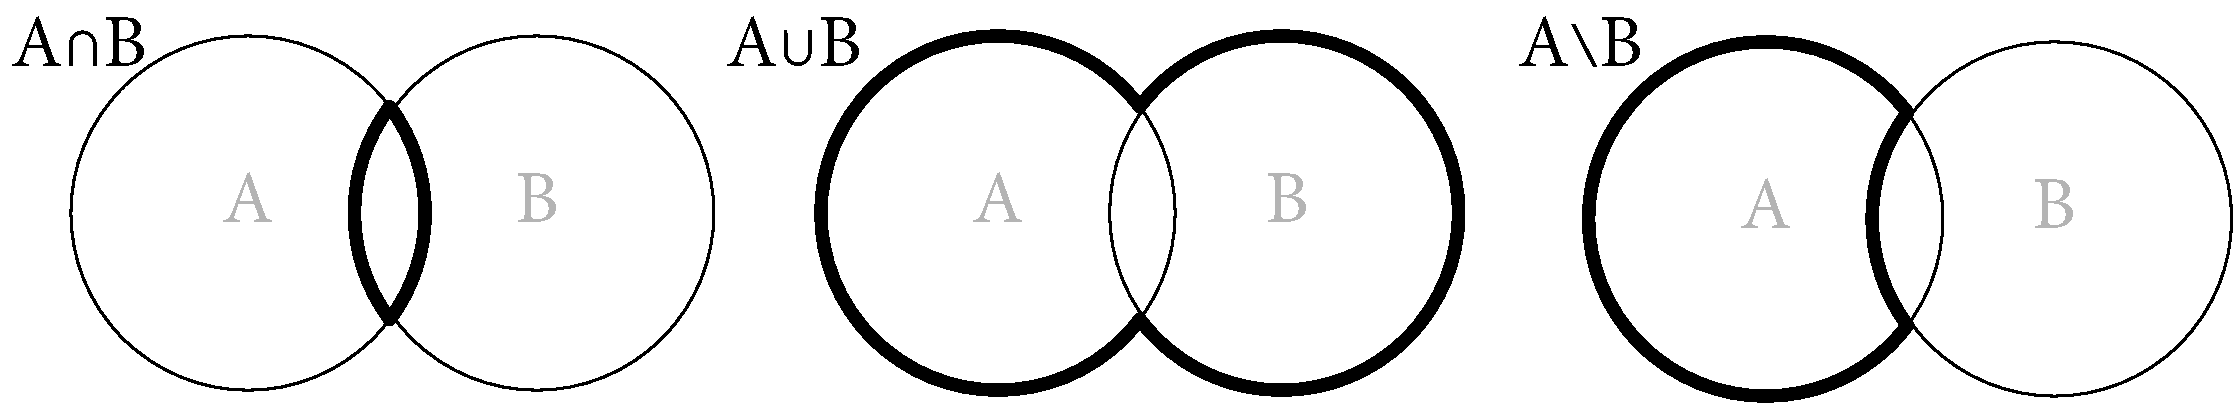
\includegraphics[width=10cm]{pic/VennMulti.pdf}
\end{center}
\caption{Intersection, Union, and Difference}
\label{figvennmulti}
\end{figure}

\begin{figure}[t]
\begin{center}
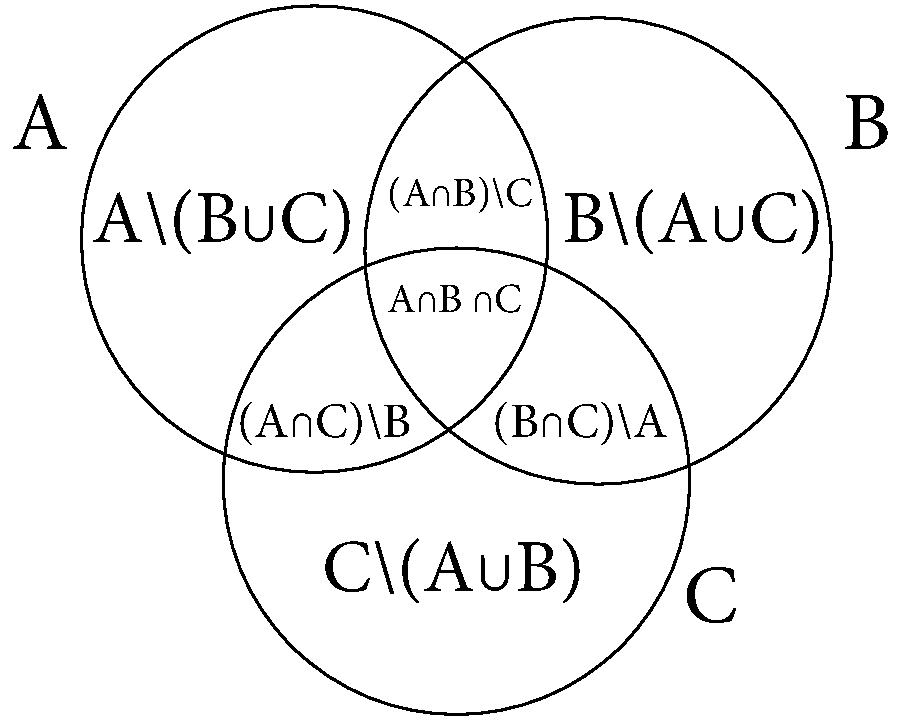
\includegraphics[width=6cm]{pic/VennDiagram.pdf}
\end{center}
\caption{A Venn diagram for three sets}
\label{figvenndiag}
\end{figure}

We observe the following basic relations for these operations:
\begin{lemma}
Let $A,B,C$ be sets. Then
\begin{enumerate}
\item $A\cap B=B\cap A$.
\item $A\cup B=B\cup A$.
\item $A\cap B\subset A$.
\item $A\subset A\cup B$.
\item $A\setminus B\subset A$.
\item $(A\setminus B)\cup (A\cap B)=A$.
\item $(A\setminus B)\cap (A\cap B)=\emptyset$.
\item $(A\cap B)\cap C=A\cap (B\cap C)$ (so we can write $A\cap B\cap C$
without ambiguity).
\item $(A\cup B)\cup C=A\cup (B\cup C)$ (so we can write $A\cup B\cup C$
without ambiguity).
\end{enumerate}
\end{lemma}

The following properties are not obvious, but can be easily seen in a Venn
diagram:
\begin{thm}[Distributive laws]
Let $A,B,C$ be sets. Then (Figure~\ref{figvenndist}):\\
a) $A\cap (B\cup C)=(A\cap B)\cup(A\cap C)$.\\
b) $A\cup (B\cap C)=(A\cup B)\cap(A\cup C)$
\end{thm}
Note that these rules mimic what happens if we multiply by a sum: $a(b+c)$.
\begin{proof}
Since we have to show equality of sets, we need to show two-sided subset
inclusion.\\
a) We show first that $A\cap (B\cup C)\subset (A\cap B)\cup(A\cap C)$: For this,
let $x\in A\cap (B\cup C)$. This means that $x\in A$ and also $x\in B$ or
$x\in C$. In the first of these cases we have that $x\in A\cap B$, in the
second that $x\in A\cap C$. Thus in either case $x\in (A\cap B)\cup (A\cap
C)$. \\
For the reverse inclusion,
let $x\in (A\cap B)$. Then $x\in A$ and $x\in B\subset B\cup C$, so $x\in
A\cap (B\cup C)$. Similarly (swap $B$ and $C$) we see that $x\in A\cap C$
implies $x\in A\cap (B\cup C)$ as well. This show that
$A\cap (B\cup C)\supset (A\cap B)\cup(A\cap C)$.

b) Exercise
\end{proof}

\begin{figure}[t]
\begin{center}
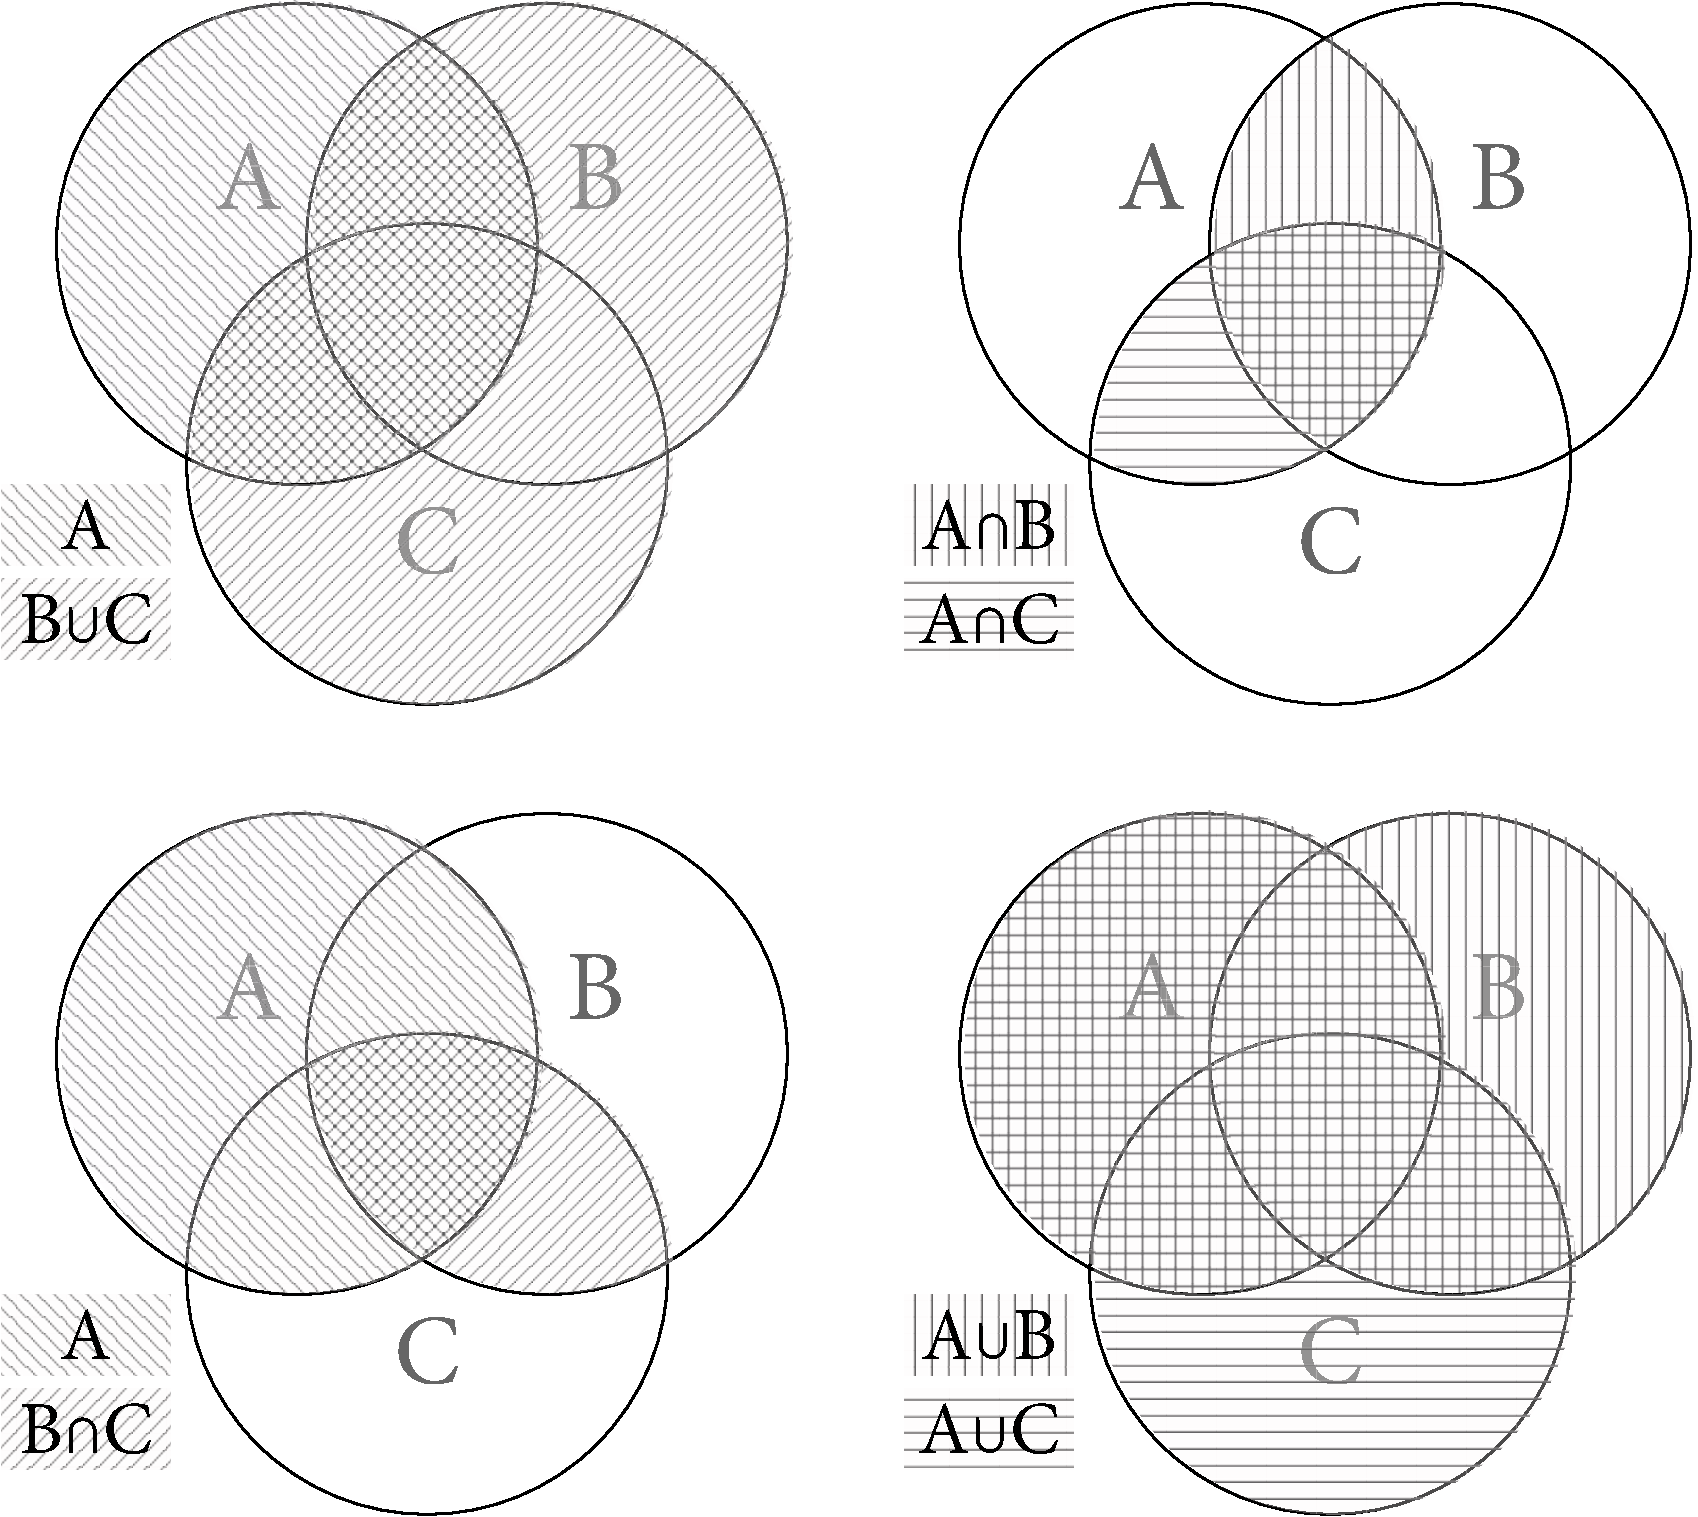
\includegraphics[width=6cm]{pic/VennDistributiveLaws.pdf}
\end{center}
\caption{Distributive Laws for Union and Intersection}
\label{figvenndist}
\end{figure}

\begin{figure}[t]
\begin{center}
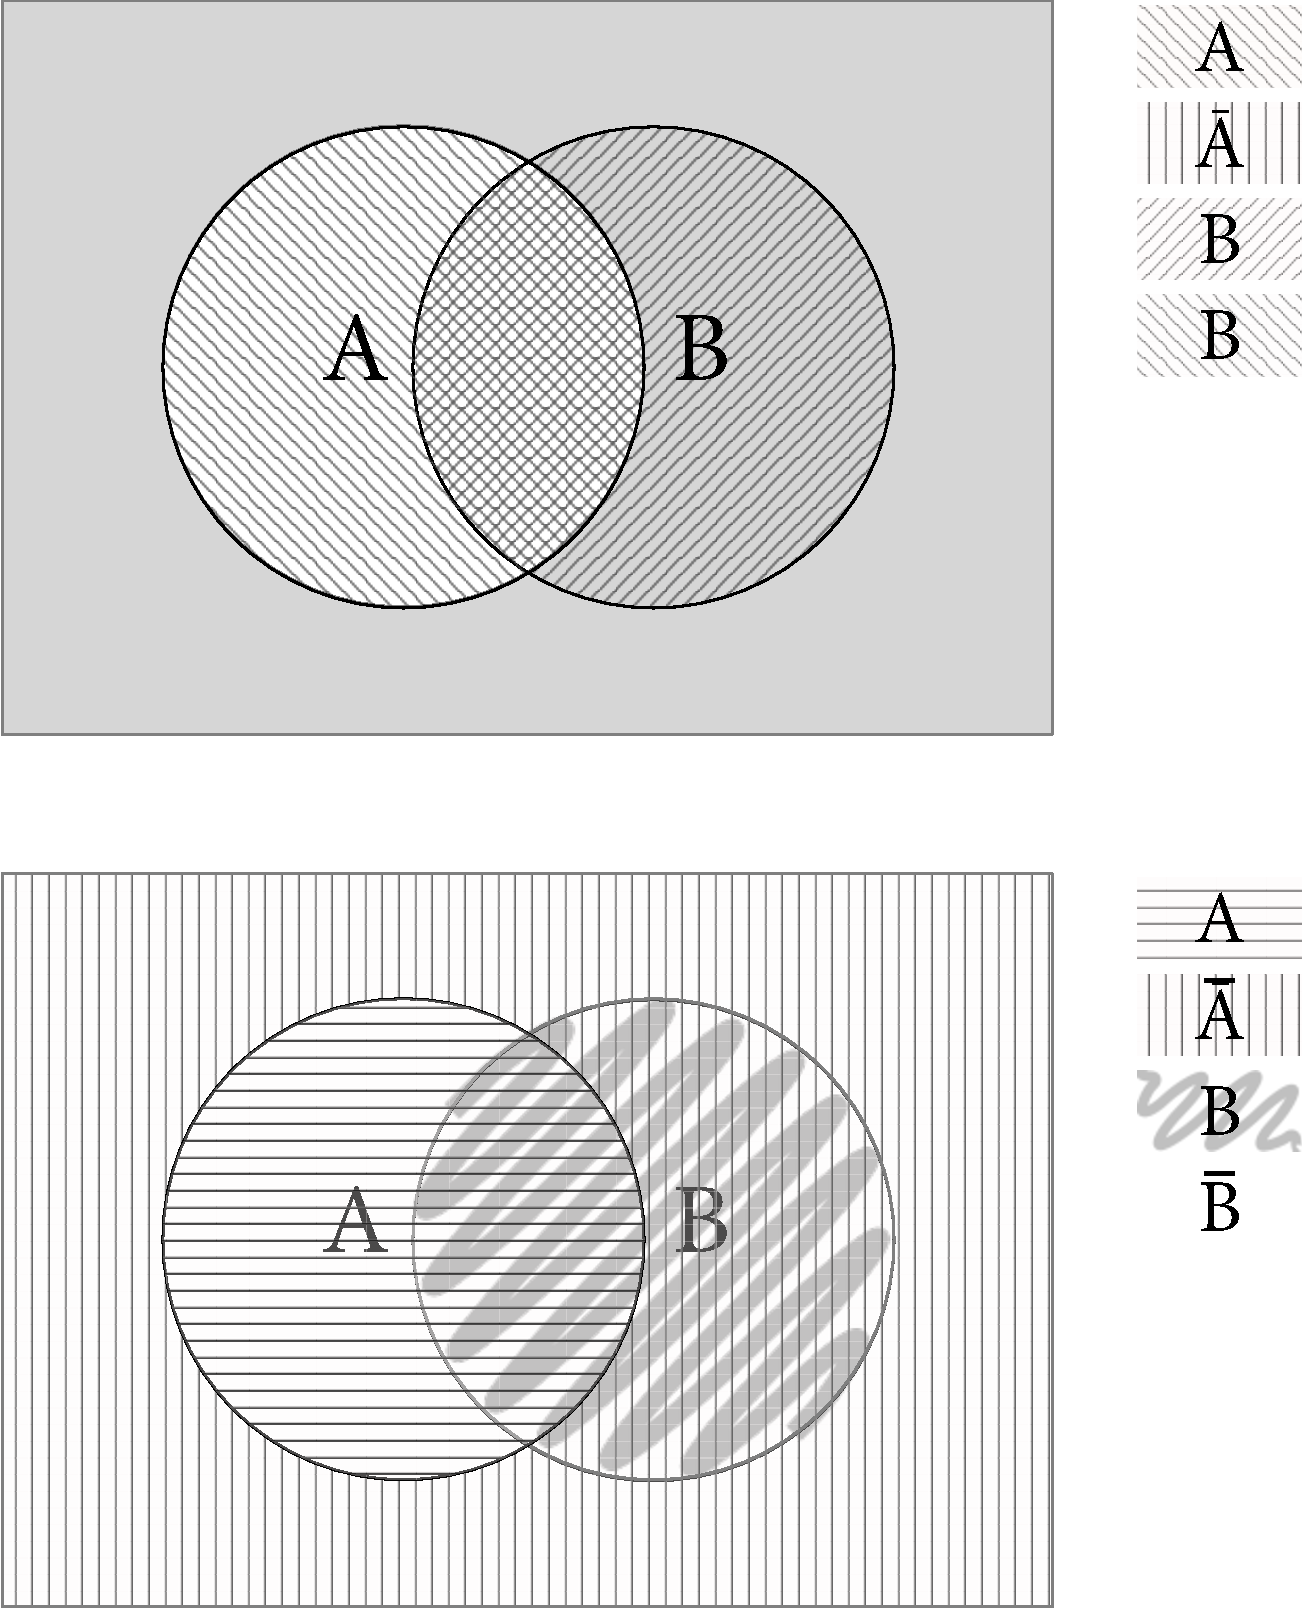
\includegraphics[width=6cm]{pic/VennDeMorganLaws.pdf}
\end{center}
\caption{De Morgan's Laws for Sets}
\label{figdemorganset}
\end{figure}

\begin{thm}[De Morgan's laws]
Let $A,B,C$ be sets with $A,B\subset C$. For any subset $D\subset C$ we
write $\overline{D}=C\setminus D$. Then (Figure~\ref{figdemorganset}):\\
a) $\overline{(A\cup B)}=\overline{A}\cap\overline{B}$.\\
b) $\overline{(A\cap B)}=\overline{A}\cup\overline{B}$.
\end{thm}
\begin{proof}
Again, we need to show inclusion in two directions:
a) Let $x\in \overline{(A\cup B)}$. That means that $x\in C$ but $x\not\in
A\cup B$. But that means that $x$ can be neither in $A$, nor in $B$, so
$x\in \overline{A}\cap\overline{B}$. Vice versa, let $x\in
\overline{A}\cap\overline{B}$. That means that $x\in C$ but $x\not\in A$ and
$x\not\in B$, and thus $x\not\in A\cup B$. This implies that
$x\in\overline{(A\cup B)}$.\\
b) Exercise
\end{proof}

\subsection{Subsets and Logic}
The last two theorems might look very similar to statements from truth
tables, if we replace $\cap$ by $\wedge$ for ``and'' and $\cup$ by $\vee$
for ``or''\mynote{This is actually the origin of these symbols. The latin
word for ``or'' is ``vel''.}. Indeed, we can translate between the two
worlds, if we imagine two properties (``predicates''), $P$, $Q$, $R$ that can
be true or false for elements in a large set. Let $A$ be the set of all
elements for which $P$ is true and $B$ the set of elements for which $Q$ is
true. Then $\overline{A}$ is the set of elements for which $P$ is false (or
$\lnot P$ is true) and so on. We thus get the logic laws:
\begin{enumerate}
\item $P\wedge (Q\vee R)=(P\wedge Q)\vee(P\wedge R)$. 
\item $P\vee (Q\wedge R)=(P\vee Q)\wedge(P\vee R)$. 
\item $\lnot(P\vee Q)=(\lnot P)\wedge (\lnot Q)$.
\item $\lnot(P\wedge Q)=(\lnot P)\vee (\lnot Q)$.
\end{enumerate}
Exercise: Sentences

We close this section with the observation that these rules can be iterated
to convert any logical expression into what is called \defini{disjunctive
normal form}, that is a sequence of blocks, each consisting of statements or
their negations, combined by {\em and}. These blocks then are combined by
{\em or}. For example:
\[
(\lnot A\wedge B\wedge\lnot C)\vee (A\wedge B)\vee (\lnot B\wedge \lnot C).
\]
(A method that is guaranteed to produce a {\em minimal} such representation
is called the {\em Quine-McCluskey algorithm}.)

\section{Building objects from sets}
\label{secmultiset}

The somewhat ``socialistic'' properties of sets -- all elements play the
same role -- might seem to be rather restrictive. Since it is possible to
put {\em anything} into a set, even other sets, it is possible to use the
construct of sets to build more complicated structures. Of course there is
nothing stopping us to introduce further notation to simplify how we write
down such objects.

\subsection{The natural numbers}

\bonussection
You might\mynote{Mirroring a famous comment by the mathematician \person{Kronecker}:
{\em God made the integers, all else is the work of man}} think
that the natural\mynote{Some people make a distinction whether $0$ should be
included. We don't} numbers, $0,1,2,3,4,\ldots$ to not require any further
introduction, but it might be illustrative how one could ``construct'' them
from (indeed) scratch:

We start with the empty set $\emptyset=\{\}$ and
denote it by $0$. Next we form the set containing the empty set:
$\{\emptyset\}$ \mynote{This is a different object, a bag with a cat in is
different from a cat!}. We call this object $1$. Next we form the set containing this
object $1$, which is $\{1\}=\{\{\emptyset\}\}$ and call it $2$ and so on.

We thus can create infinitely many objects, called $0,1,2,\ldots$. We call the
collection of these objects (which really all are sets, of varying nestedness) the
\defini{natural numbers}, and write them as $\N$.

Furthermore, if $n$
is such an object, we can define an addition by 1 as giving the result $\{n\}$. From
this, it is possible to construct addition of arbitrary objects as follows:

Let $m,n\in\N$. If $n=\emptyset$, define $m+n=m$. Otherwise (that is, if
$n\not=\emptyset$, that is $n=\{x\}$ for some other $x=n-1\in\N$), define addition
recursively by
\[
m+n=(m+1)+x=\{m\}+x.
\]
(we yet lack the formal tools to prove that this defines a proper addition structure).

\subsection{Pairs and Tuples (or lists)}

In many situations, we care not just about multiple objects being together in a set,
but want to designate particluar objects\mynote{E.g. a designated driver} in a set as
being special. We could do so, using only the data structure of sets, by similarly
wrapping objects into sets: The sequence $a,b,c$ can be represented by the set
$\{\{1,a\},\{2,b\},\{3,c\}\}$.

\begin{quote}
\bonussection
You might spot a difficulty in this plan. What if -- say -- $a=2$ and $b=1$ and the
sets $\{1,2\}$ and $\{2,1\}$ become the same. We could avoid this, by wrapping the
numbers, together with the empty set to avoid confusion with the construction of the
natural numbers, into a set and thus store
\[
\{\{\emptyset,1\},a\},\{\emptyset,2\},b\},\{\emptyset,3\},c\}\}.
\]
This still can cause problems if -- say -- $b=\{\emptyset,1\}$. One thus needs to
replace $\emptyset$ by an object that is different from anything else used. Again we
won't go into the technical details of this.
\mynote{In practice, of course you will not need this convoluted construction, but can
simply write $(a,b)$.}
\end{quote}

We will typically put parentheses (or brackets) around objects to write down such an
ordered collection: $(a,b,c)$ or $[a,b,c]$. We call these objects \defini{tuples}. So
for example $(7,3,5)$ is a $3$tuple and $(8,2,5,1,4,1,2)$ an $7$-tuple. In the special
case of $2$-tuples we call such objects simply \defini{pairs}.
\smallskip

If we have two sets $A,B$, we sometimes want to describe the set of all possible pairs.
This set is called the \defini{cartesian product}\mynote{Named after the French
mathematician \person{Ren\'e Descartes}, who invented the standard $x/y$ coordinate set,
the \defini{Cartesian coordinates}, in which points are described by pairs.} of $A$ and
$B$ and written as
\[
A\times B=\{(a,b)\mid a\in A,b\in B\}
\]
For example, if $A=\{1,2,3\}$ and $B=\{5,6\}$, then
\[
A\times B=\{(1,5),(1,6),(2,5),(2,6),(3,5),(3,6)\}
\]

It is easy to see that if $\sz{A}=m$ and $\sz{B}=n$, then $\sz{A\times B}=m\cdot n$.

Of course arbitrary $k$-tuples can be descibed in the same way by an iterated cartesian
product $A\times B\times C\times\cdots\times K$.

\subsection{Indexing and index sets}

If we have a $k$-tuple we call $t$, we might need to refer to a particular entry
of the tuple in a particular position. We do so by writing the position number as an
\defini{index}, that is a number put on the bottom right of the object. That is the
$5$-th entry of the tuple $t$ would be denoted by $t_5$ and if we write out elements we
will have
\[
t=(t_1,t_2,\ldots,t_k).
\]
There is nothing stopping us to index by a variable and denote the $i$-th element of
the tuple $t$ as $t_i$.

If we consider all entries of a $k$-tuple, we might want to use an
\defini{index set}: Let $I=\{1,2,\ldots,k\}$ and we will talk about $t_i$
for $i\in I$.  \mynote{The reader who already has some programming
experience should think at this point of a \texttt{for}-loop. The $i$ (for
``index'') from mathematics is also the reason, that the standard name of a
loop variable is \texttt{i} as well.}

This concept (and notation) generalizes easily to other, even infinite index
sets. We might take an index set $P$ of persons ans then talk of the first
name $f_p$ for a person $p\in P$. Or we look at entries $t_i$, $i\in\N$ for
an infinite tuple.

\subsection{Multisets}

We can use the construct of an index set to associate counts to objects of a
set and thus represent objects being in a set multiple times. The resulting
object is called a \defini{multiset}. Formally, a multiset can be defined as
an ordinary set $S$, together with a counting set $C=\{c_s\in\N\mid s\in
S\}$ indexed by $S$. This pair $(S,C)$ then represents a collection in which
object $s\in S$ occurs  $c_s$ times. For example, we could describe a
wallet's content by the set $S=\{p,n,d,q\}$ \mynote{US-centric {\em
penny},{\em nickel} (5 cent),{\em dime} (10 cent), {\em quarter} (25 cent).}
and have e.g. 
\[
W=(S,C),\quad C=\{c_p=3,c_n=1,c_d=0,c_q=3\}.
\]

\subsection{Why only sets}

\bonussection
Given the contortions we just performed to construct more complex objects
from sets, the reader might wonder about why we did so? The reason is to
simplify construction (and requirements in proving that certain
constructions are valid and consistent -- though we won't be doing this in
this course): If everything is a set, we only need to handle sets, and won't
need to do the same thing for multiple different constructs.

That is, as far as mathematics is concerned. If you store data in a program,
it of course would be wasting space and processing time  by building
convoluted iterations of sets. Instead -- and this is one of the core
concepts of computer science -- it will be necessary to devise more
efficient (in terms of storage, and of access time and functionality) data
structures for storing a particular kind of information. One of your skills
as a computer scientist will be to bridge this translation from {\em
abstraction} in mathematics to suitably chosen data structures in a program.

\section{Some foundational caveats}

\bonussection
We have so far presented set theory as an easy-peasy, worry-free,
playground. In practice (that is with all sets you will encounter in your
professional life as a computer scientist), this is the case. But if you are
interested in the foundations of mathematics or in logic as an abstract
subject, you should be advised that, as in medieaeval maps, there are
monsters lurking in the margins which make it hard to formally prove basic
properties. To just give you an example of such problems, imagine (since
sets can contain {\em anything}) that we allow sets to contain
themselves\mynote{Picture: Dragon biting its tail}. Then we can distinguish
between sets that contain themselves, and those who do not. Now consider we
form a new set $S$, whose members are all sets that do not contain
themselves. Then, if $S$ contains itself, it should not, but if it does not
contain itself it should! 

Such questions, when first raised between about 1850 and 1920, caused significant
distress to mathematicians (which claimed to have the most rigorous foundation of all
disciplines), but today have -- at least in the author's view -- been basically
resolved (or shown to not have practical relevance).

\section{Quantifiers}

There is one more thing we shall want to do with sets, namely

\section{Relations}

In the same way that skis without slopes are of limited excitement, just
talking about individual sets will not get us very far. Instead, we want to
set different sets in relation to each other. The general concept is that of
a relation, described in this section. We later will consider functions as a
special, particularly nice, case of relations.

\begin{defn}
Let $A,B$ be sets. A \defini{relation} between $A$ and $B$ is a subset $R\subset
A\times B$, that is $R$ is a set of pairs $(a,b)$ with $a\in A$ and $b\in B$. We say
that $a\in A$ is in relation to $b\in B$ (sometimes written $a\sim_R b$ (or even just $aRb$) if and only if $(a,b)\in R$.
\end{defn}

We could for example take $A$ the set of all students and $B$ the set of all majors
with the relation describing the major(s) of every student.\mynote{Note that multiple
students might have the same major and that some students might have multiple majors.}

Another example of a relation would be $A$ the set of natural numbers and $B$ the set
of prime numbers with the relation $R$ defined as a number $a$ being in relation to a
prime $b$ if and only $b$ divides $a$. Then for example $4\sim_R 2$ but
$4\not\sim_R 3$, nor $2\sim_R 4$. Then some of the elements of $R$ are
\[
(2,2), (4,2), (6,2), (3,3), (6,3), \ldots (20,2),(20,5),\ldots \in R.
\]
Note that the relation is just what we defined. For example we have that
$(-10,2)\not\in R$ and $(12,6)\not\in R$, since neither of these two pairs would be in
$A\times B$.\mynote{One could of course extend the divisibility relation to larger sets
and then have these pairs in the new, larger, relation.}

You will have seen the concept of relations before, though maybe not under
this name.  If $A$ and $B$ are the rational numbers (or the real numbers, or
the integers), we can interpret $A\times B$ as the plane of points in a
coordinate system. Any relation $R\subset A\times B$ then can be visualized
as a set of points in the plane. We call this the \defini{graph} of the
relation.  A number of examples are shown in
\figuref{figsomeRelations}

\begin{figure}[t]
\begin{center}
%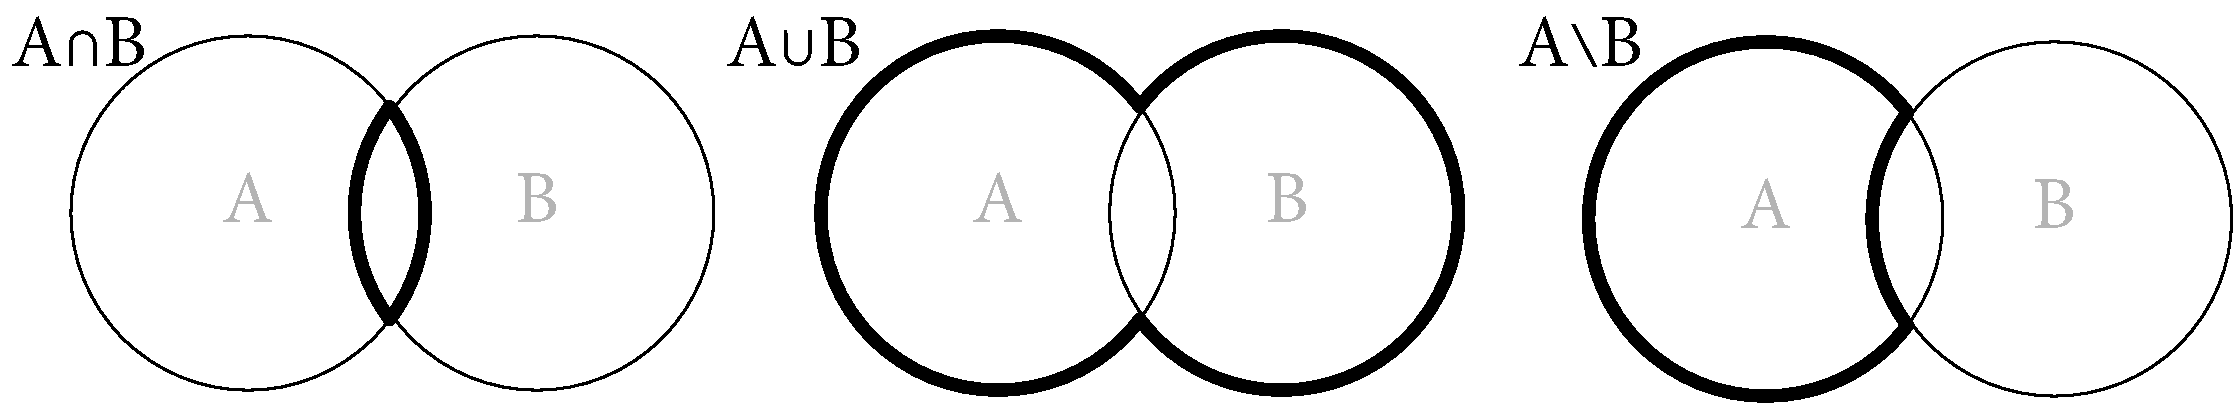
\includegraphics[width=10cm]{pic/VennMulti.pdf}
$x^2+y^2=1
y=x^2
x=y^2
y^2 = x^3 - 3*x + 1
x,y\in\Z
2\le x,y\le 3
|x-y|<1$
Smileyface
\end{center}
\caption{Some relations}
\label{figsomeRelations}
\end{figure}

If we set $A=B$ (as we did in these examples), we can use relations (in the
mathematical sense) to describe
relations (in the common language sense)  amongst the elements of that set. 
In this case, the relation is also called a \defini{binary relation} on the set, in
particular if using a notation similar to $a\sim b$.

For example, consider the well known operations $=$, $<$, $\le$ in the rational
numbers. As we will see, relations thus allow us to generalize concepts of equality or
order As we will see, relations thus allow us to generalize concepts of equality or
order. We could, for example define a relation $\sim$ on the
rational numbers by defining $a\sim b$ if $-10^{-5}<a-b<10^{-5}$. such a relation could
be used to model rounding.

We now define a number of peroperties that a binary relation could have:
\begin{defn}
Let $\sim$ be a binary relation on a set $A$. Then $\sim$ is called
\begin{description}
\item[\defini{reflexive}], if $a\sim a$ for every $a\in A$.
\item[\defini{symmetric}], if (for $a,b\in A$) $a\sim b$ implies that $b\sim a$.
\item[\defini{antisymmetric}], if (for $a,b\in A$) $a\sim b$ and $b\sim a$ together
imply that $a=b$. (This means that, apart from a trivial case we might have either
$a\sim b$ or $b\sim a$, but not both. Think of the $\le$ relation on numbers.)
\item[\defini{transitive}], if (for $a,b,c\in A$) $a\sim b$ and $b\sim c$ imply that
$a\sim c$.
\end{description}
\end{defn}
We give some examples: 
\begin{enumerate}
\item
Let $A$ be the set of rational numbers and $R$ be ordinary equality. (That is 
\[
R=\{(a,b)\in\Q\times\Q\mid a=b\}.)
\]
This relation is reflexive, symmetric and transitive
\item
Let $A$ be the set of all people in a country with two people in relation if they have
the same last name. This relation is reflexive, symmetric and transitive.
\item
Let $A$ be the set of all people living in the United States
\mynote{Constitutional
scholars should take the continental US without Washington DC here} with two people in
relation if they live in the same state. gain this relation is reflexive, symmetric and
transitive.
\item
\label{expointpairs}
Let $A=\R\times\R$ the set of points in the plane, with two points in relation
if they have the same $x$ coordinate or the same $y$ coordinate. (That is, one could
draw a horizontal line or a vertical line through the two points.)
We practice the set notation for relations by writing this down formally, noting that
we have to describe pairs of pairs:
\[
R=\{((x,y),(a,b))\in A\times A\mid x=a \mbox{\ or\ }y=b\}.
\]
This relation is reflexive and symmetric, but not transitive (go first horizontal, then
vertical).
\item
We slightly modify example~\ref{expointpairs} by requiring same $x$ or same $y$
coordinate, but not both the same. Then the relation is only symmetric, but not
reflexive any more.
\item
Let $A$ be a set and $R=A\times A$ (i.e. all elements are in relation). This relation
is reflexive, symmetric and transitive.
\item
Let $A$ be an arbitrary nonempty set and $R=\emptyset$ (that is no elements are in
relation). Then $R$ is symmetric and transitive (both conditions are vacuously true
since they are ``if-then'' with a condition that never can be fulfilled), but not
reflexive.
\item Let $A=\Q$ with the usual ``smaller or equal'' relation $\le$. This relation is
reflexive, antisymmetric and transitive, but not symmetric.
\item Let $A=\Q$ with the ``strictly smaller'' relation to be smaller but not equal. 
This relation is antisymmetric (again vacuously as it is not possible that $a<b$ and
$b<a$ for inequal $a,b$) and transitive, but not reflexive.
\item The relation $x^2+y^2=1$ on $\R$ has none of these properties.
\end{enumerate}

EX:What does it mean for the graph if reflexive etc.

\section{Equivalence Relations, Partitions}

We now consider relations that could be used to define equality. This is a
concept you have used before without trouble. For example you probably would
claim that $3=\mbox{\Huge 3}$, even though the digits are of different
size\mynote{On the other hand, if your business is selling house numbers,
you might consider them different, as you will be charging more for the
larger digit.}. But they represent the same. Some of the examples in the
last section share this characteristic.
\begin{defn}
A binary relation $\sim$ on a set $A$ is an \defini{equivalence relation} if
it is reflexive, symmetric and transitive.
\end{defn}
Equivalence relations can be though of as a `less picky'' version of
equality that allow us to forget about differences between objects (say the
color of numbers), that are irrelevant for what you are doing. If you say
that $1+1=2$ you use an equivalence relation on algebraic expressions ($1+1$
and $2$) that a typesetter would not make.

An important characterization of equivalence relations is that they chop a
set into parts.
\begin{defn}
Let $A$ be a set. A \defini{partition} of $A$ is a set $P$ consisting of nonempty
subsets of $A$, such that:
\begin{enumerate}
\item No two different subsets share an element\mynote{This is a somewhat slick
definition. You probably would have written ($S=T$ or $S\cap T=\emptyset$). This would
describe the same (logic), but the way we write it down here make verifying the property
less work to write.}:
\[
\forall S,T\in P: (S\cap T\not=\emptyset\Rightarrow S=T).
\]
\item Every element of $A$ is in a subset: 
\[
\forall a\in A\exists S\in P: a\in S.
\]
\end{enumerate}
\end{defn}
For example, we could take $A=\{1,2,3,4,5\}$ and 
\[
P=\{\{1,3\},\{2,4,5\}\}.
\]
\begin{lemma}
Let $P$ be a partition of $A$. Then every element of $A$ is in exactly one $S\in P$.
\end{lemma}
\begin{proof}
By the second property it needs to be in at least one set, by the first property it
cannot be in more than one.
\end{proof}

Given a partition $P$ of $A$, this allows us to define a relation on $A$ by
defining $a\sim b$ if and only if $a$ and $b$ are in the {\em same} set of
the partition. In the example above, this would yield the relation
\[
\{(1,3),(3,1),(2,4),(4,2),(2,5),(5,2),(4,5),(5,4)\}
\]
Such a relation is clearly an equivalence relation: An element is in the
same set as itself. If $a$ and $b$ are ih the same set, so are $b$ and $a$,
and if $a$ and $b$, as well as $b$ and $c$ are in the same set, this set
contains $a$ and $c$.

The same holds in reverse. For this, assume we are given an equivalence
relation $\sim$ on a set $A$. For every $a\in A$ we 
define its \defini{equivalence class} as the set of all elements in relation
to $a$:
\[
[a]=\{b\in A\mid b\sim a\}.
\]
Clearly $a\in[a]$ is in its own equivalence class, and equivalence classes
thus are not empty, and every element of $A$ lies in an equivalence class.
We also note that if $a\sim b$, then $[a]=[b]$, since any $c\in[a]$
satisfies $c\sim a$ and thus $c\sim b$ by transitivity (and vice versa for
$c\in[b]$). Thus, if two equivalence classes intersect nonempty, they are
equal: Let $c\in [a]\cap [b]$, then $c\sim a$, $c\sim b$ (and thus $b\sim c$
because of symmetry) and by transitivity $b\sim a$ and thus $[a]=[b]$.

This means that the set of equivalence classes forms a partition of the set
$A$.

In the above example, the relation 
\[
\{(1,3),(3,1),(2,4),(4,2),(2,5),(5,2),(4,5),(5,4)\}
\]
creates the equivalence classes
\[
\{1,3\}\mbox{\ and\ }\{1,4,5\},
\] and thus the partition $P$.

For another, prototypical, example, suppose we define a relation $\sim$ on the set $\Z$ of
integers by defining $a\sim b$ if $2$ divides $a-b$. Then we get two
equivalence classes, namely the even and the odd numbers. If we change the
equivalence to $a-b$ being divisible by $3$, we get three
(infinite) equivalence classes:
\[
\{0,3,-3,6,-6,\ldots\},\quad
\{1,4,-2,7,-5,\ldots\},\quad
\{2,5,-1,8,-4,\ldots\}.
\]
Equivalence classes will be important tools for us to construct new classes
of objects, in particular arithmetic objects.

For a more elaborate example of equivalence classes, and why we care about
them, consider graphs. A graph consists of \defini{vertices} (basically
points), together with \defini{edges} that each connect two vertices.

To represent a graph, we need to represent the vertices -- say for a graph
on $n$ vertices with the numbers $1,2,\ldots,n$. An edge then is a set of
two vertices. For example (\figuref{3vertexgraphs}) consider graphs on $n=3$
vertices. There are 3 potential edges and each edge can be selected or not,
so we get $2^3=8$ possibilities for \defini{labelled graphs}, that is graphs
where the labelling of the vertices matters.

But often we do not care about this labelling but only  about the possible
connection patterns. We thus can define an equivalence relation
(called~\defini{graph isomorphism}) as two graphs becoming the same after a
relabelling of the vertices. For example, the graph with the edge set
$\{\{1,2\}\}$ can be trandformed into the graph with edge set $\{\{2,3\}\}$ by
relabelling
\mynote{This is not unique. Another opion would be $\begin{array}{c}1\to
3\\2\to2\\3\to1\end{array}$.} 
the vertices $\begin{array}{c}1\to 2\\2\to3\\3\to1\end{array}$.

We thus get (for the example of three vertices) $4$ equivalence classes
(as indicated by shaded areas in the figure). These equivalence classes are
what we consider typically as (unlabelled) graphs. 

\section{Order Relations}

\section{Functions}

Functions are arguably at the heart of mathematics and are the most
important definition of the whole course.

A \defini{function} is a relation $R$ with the special property that there
are no two pairs $(a,b),(a,c)\in R$ that share the same first entry.  If
this is the case, we can interpret the relation entry $(a,b)\in R$ (which
will be the only one for a given $a$) as {\em assigning} the value $b$ to
$a$.

\begin{defn}
Let $A,B$ be sets and $R\subset A\times B$ a relation. Then $R$ is called
a~\defini{function}, if for all $a\in A$ and $b,c\in B$, if $(a,b)\in R$ and
$(a,c)\in R$, then $b=c$.
We call  (see \figuref{figgeneralfct} for illustration)
\[
D=\{a\in A\mid \exists b\in B: (a,b)\in R\}
\]
the \defini{domain} of $R$ and
\[
I=\{b\in B\mid \exists a\in A: (a,b)\in R\}
\]
the \defini{image} of $R$, and $B$ the \defini{codomain} (sometimes called
the \defini{range}) of $R$.

For $a\in D$, we call $R(a)=b$, for $b\in B$
the unique element with $(a,b)\in R$, the \defini{value} of $R$ at $a$, or
the \defini{image} of $a$ under $R$.
\end{defn}

\begin{figure}[t]
\begin{center}
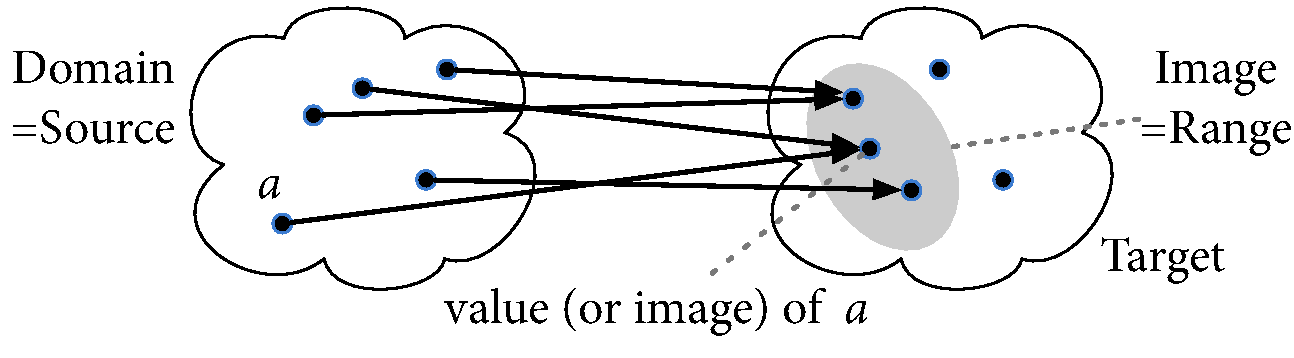
\includegraphics[width=6cm]{pic/GeneralFct.pdf}
\end{center}
\caption{A function}
\label{figgeneralfct}
\end{figure}

In short, a function is a rule that assigns for every element of its domain
an element of its codomain.

Sometimes the term \defini{map} or \defini{mapping} is used synonymously
with {\em function}.


For relations on $\Q,\R$ (or subsets thereof), the condition can also be
visualized in the graph if the relation by the property that no two points
of the relation lie on a vertical line. In the examples in
\figuref{figsomeRelations}, the relations under XXX are functions, the others
are not.

Two functions are equal if they have the same domain, the same codomain, and
(and this is the most important property)
if they assign to every element of the domain the same value.
\method{Equality of functions}
To show that two functions $f,g$ are equal, we need to compare their
domains, their codomains, and finally show that for every $x$ in the domain
we have that $f(x)=g(x)$.

\subsection{Describing Functions}

In most cases, functions are easiest given not as a relation (or by their
graph), but using the interpretation of assigning values to elements of
their domain.
Typically a function is specified, by
giving its domain, its codomain, and a rule that specifies the value of the
function for every element of the domain. This value must be an element of
the codomain.

A function can be specified by text, formula, table, case distinction, picture,
algorithm, to name just a few ways. Concretely, we write the name of the
function, a colon $\colon$, the domain, an arrow, and the codomain. If the
value is given by a formula, often the notation $a\mapsto \mbox{formula}(a)$
is used. In many cases, it is convenient to describe a function informally
by text and makes for easier understanding. On the other hand, a formal
description avoids ambiguity and often makes it easier to formally prove
statements. Finally formal definitions are often easier to implement of a
computer.

The following thus are all perfectly good definitions of functions:
\begin{enumerate}
\item  Let $A=\{\mbox{frog},\mbox{horse},\mbox{sheep}\}$ and $B$ the set of
colors. We define $f_1\colon A\to B$ by assigning to each animal its outer
color:
\[
f_1\colon \left\{\begin{array}{lcl}
\mbox{frog}&\to&\mbox{green}\\
\mbox{horse}&\to&\mbox{brown}\\
\mbox{sheep}&\to&\mbox{black}\\
\end{array}
\right..
\]

\item Another function $f_2$ with same domain and codomain might assign to each animal its favorite color, say
\[
f_2\colon \left\{\begin{array}{lcl}
\mbox{frog}&\to&\mbox{green}\\
\mbox{horse}&\to&\mbox{red}\\
\mbox{sheep}&\to&\mbox{blue}\\
\end{array}
\right..
\]
This same function $f_2$ could be specified as
\[
f_2\colon a\to\left\{\begin{array}{ll}
\mbox{green}&\mbox{if $a=$frog,}\\
\mbox{red}&\mbox{if $a=$horse,}\\
\mbox{blue}&\mbox{if $a=$sheep.}\\
\end{array}
\right.
\]
Or someone might draw the function pictorially, as in
\figuref{figfroghorsesheep}.
\begin{figure}[t]
\begin{center}
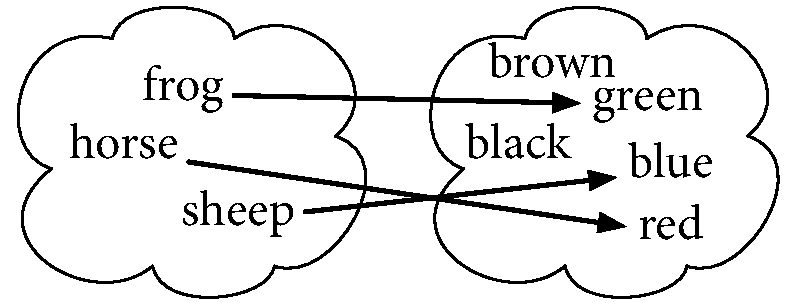
\includegraphics[width=6cm]{pic/AnimalColor.pdf}
\end{center}
\caption{A function assigning colors to animals}
\label{figfroghorsesheep}
\end{figure}
\item 
\item Let $A$ be the set of students at this university and $B$ the set of
symbol strings. The function $f_4\colon A\to B$ assigns to each student
their email password. (It is a function, even though only each
student is supposed to know their function value.)
\item Let $D$ be the set of days of the current year and $T$ the set of
minutes in a day. We define the ``sunrise time in Denver'' function $f_5\colon
D\to T$ as assigning to each date the time of sunrise (in Denver, CO).
\item Let $S$ the set of students in this class and $G$ the set of grades.
Define $f_6\colon S\to G$ the function that assigns each student the
grade they will obtain in the class.
(To be a function, it is only required that the value is unique and
unambiguous, not that it is easily computable or known at the moment)
\item For $A=\N$ the set of nonnegative integers,
let $f_7\colon A\to A$, $x\mapsto x+1$. Other examples would be
$f_8\colon A\to A$, $x\mapsto x$, or
$f_9\colon A\to A$, assigning to $x$ the number of digits $x$ requires in
decimal representation.\mynote{You might note that we could alternatively
write $f_9(x)=\lfloor\log_{10}(x)\rfloor+1$, using the $\lfloor\cdot\rfloor$
notation for truncation.}
\item Let $f_{10}\colon \R\to\R$, $x\mapsto\frac{x^3+x+1}{x^2+1}$.
\item Left $f_{11}\colon\R\to\R$, $x\mapsto\begin{cases}
1&x<0\\
-2&x=0\\
x+17&0<x<1\\
\cos(x)&x\ge 1\\
\end{cases}$.
\item Let $g\colon\N\to\Q$ to give for each $n$ the first $n$ decimal
places of $\pi$. Thus $g(0)=3$, $g(1)=3.1$, $g(2)=3.14$ and so on. If we go
back to the notation of relations, we get
\begin{eqnarray*}
g&=&\{(n,\mbox{$\pi$ to $n$ decimal digits}\}\\
&=&\{(0,3),(1,3.1),(2,3.14),(3,3.141),(4,3.1415),\ldots\}.
\end{eqnarray*}
\end{enumerate}

On the other hand, the following attempts do not define functions (for
reasons indicated).
\begin{enumerate}
\item The relation $R=\{(a^2,a)\mid a\in\Q\}\subset\Q\times\Q\}$ is not a
function, {\em since there are multiple elements in $R$ -- e.g. $(4,2)$ and
$(-4,2)$ with the same first entry, so images are not uniquely defined.}
\item
Let $f\colon\Q\to\Z$ assigning to every rational number the
closest integer. {\em Not a function, as the closes integer is ambiguous,
say for $1/2$.} We can fix it, by defining an explicit tie-break rule for
ambiguous cases. What is often used is to take the largest integer $\le
x+\frac{1}{2}$.
\item
Let $f\colon\Q\to\Q$, $x\mapsto{x^2-1}{x-1}$. {\em This is not a function,
as the denominator at $x=1$ becomes zero.} One could fix it by changing the
domain to $\Q\setminus\{1\}$, or by replacing it with the function $x\mapsto
x+1$ (which for all $x\not=1$ returns the same value).
\item
Let $f\colon\Q\to\Q$, $x\mapsto\sqrt{2}$. {\em Not a function, as values,
such as $\sqrt{2}$ are not rational, and for negative $x$ are not clearly
defined.}
We can fix this by changing the domain to $\Q_{\ge 0}=\{a\in\Q\mid
a\ge 0\}$ and the codomain to $\R$.
\item Assigning to every subset of the rational numbers its smallest
element. {\em Not a function, since e.g. the set $\{a\in\Q\mid a>0\}$ has no
smallest element.} We can fix this using concepts from
limits\pointer{seclimits}.
\end{enumerate}


\subsection{Functions of several variables}

Binary operations

\subsection{Functions in programming}

\section{Properties of Functions}

Restriction

\section{Composition}

\section{Inverse Functions}

\section{Counting}

\chapter{Arithmetic}

In this chapter we will describe multiple flavours of numbers that will be
useful. You probably have encountered most (or even all) of these sets
before, but our approach will most likely be different from what you have
done before:
\begin{enumerate}
\item We shall describe a construction of these numbers (and their
arithmetic), starting with the natural numbers.
\item For those interested in working with numbers on the computer, we will
contrast the mathematical construction with how one could implement such
objects on the computer.
\item
These constructions serve as examples for some of the constructs, in
particular equivalence classes, which we defined earlier.
\end{enumerate}

We assume that the natural numbers
\[
\N=\{0,1,2,3,\ldots\}
\]
are being given, together with an addition $+$. We define subtraction by
setting, for $a\ge b$, $a-b$ to be the number $c$ such that
$b+c=a$.\mynote{To make this logically solid, we would have to prove that such
an element $c$ is unique.}

\section{Integers}


\begin{defn}
For integers $a,b\in\Z$, we say that $a$ \defini{divides} $b$ (written
$a\mid b$) if there
exists a $c\in Z$ such that $b=ac$. In symbols, 
\end{defn}

\subsection{Division with Remainder, Euclidean Algorithm}

Probably the most important property of the integers, and the one from which
many of its properties follow, is division with remainder. 

An important  consequence of this is the unique factorization into prime numbers

\begin{defn}
An integer $p\in\Z\setminus\{-1,0,1\}$ is called a \defini{prime} number, if
the only divisors of $p$ are $\pm 1$ and $p$ itself.
\end{defn}
Typically we consider only positive prime numbers (and call the negative
prime numbers \defini{associated}).
\begin{lemma}
Let $p$ be a prime number and $a,b\in Z$ such that $p\mid ab$. Then $p\mid
a$ or $p\mid b$.
\end{lemma}
\begin{proof}
If $p$ does not divide $a$, then
If $p$ divides neither $a$, nor $b$, we can write $a=qp+r$, $b=sp+t$ with
$0<r,t<p$ nonzero. Then
\[
ab=(qp+r)(sp+t)=\underbrace{qsp^2+qpr+srp}_{\mbox{multiples of $p$}}+rt
\]
\end{proof}
\begin{cor}
Every integer $n$ can be written uniquely as a product
\[
n=\pm1\cdot p_1^{e_1}p_2^{e_2}\cdots p_k^{e_k}=\prod_{i=1}^k p_i^{e_i}
\]
where the $p_i$ are distinct, nonnegative, prime numbers with $p_i<p_{i+1}$
(so the arrangement of the $p_i$ is fixed) and positive integral exponents
$1\le e_i$.
\end{cor}
The proof is not hard: take two factorizations and consider a prime factor
in one of them. By the lemma, it must divide a prime factor in the other
factorization, and thus be equal. However writing it down formally 



\subsection{Flashback: Polynomials}
\bonussection

If you think back at Algebra class in middle school ...

\section{Modular Arithmetic}

\section{Rational Numbers}

\section{Real Numbers}

You should read this section only after ...

\subsection{Algebraic Expressions}

\section{Complex Numbers}

\subsection{Polar Form}

\section{Polynomials}

\subsection{Rational Functions}

\subsection{projections}
POWERSET

\begin{figure}[t]
\begin{center}
%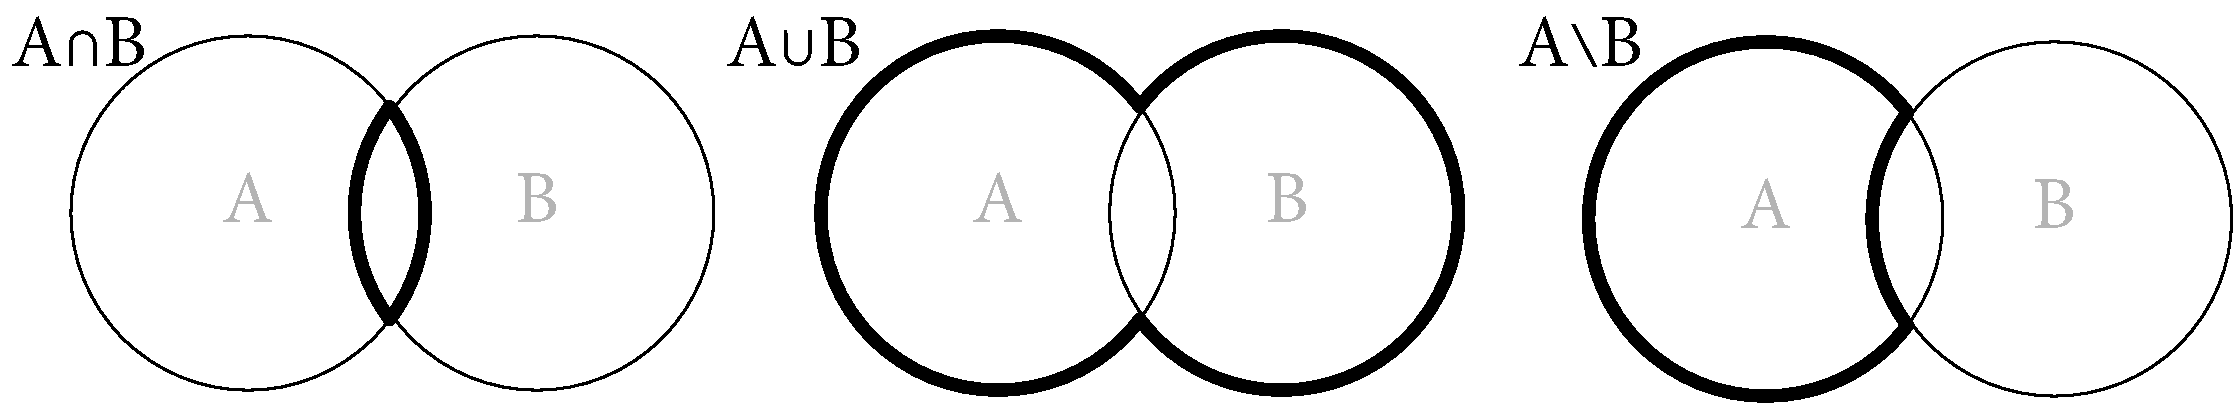
\includegraphics[width=6cm]{pic/VennMulti.pdf}
\end{center}
\caption{Title}
\label{figlabel}
\end{figure}
